\section{Технологический раздел}
\label{sec:technology}

\subsection{Выбор технологий для реализации системы}

Были выбрали надежный и современный набор технологий для своего веб-сервиса «Бюро находок». Вот краткий обзор некоторых из наиболее важных технологий в вашем стеке и почему они полезны для проекта:

\begin{enumerate}
	\item Next.js~--- это мощная платформа React, которая обеспечивает рендеринг на стороне сервера и генерацию статических сайтов, что может помочь улучшить производительность и SEO веб-приложения. Он также поддерживает маршруты API, что упрощает внутреннюю разработку в рамках одного проекта~\cite{bib:nextjs}.
	
	\item React~--- популярная библиотека JavaScript для создания пользовательских интерфейсов, особенно одностраничных приложений, где требуется быстрый ответ на взаимодействие с пользователем. Это помогает в создании повторно используемых компонентов пользовательского интерфейса~\cite{bib:reactjs}.
	
	\item tRPC позволяет создавать типобезопасные API без необходимости писать схемы или генерировать типы. Он использует TypeScript, чтобы обеспечить проверку типов входных и выходных данных API, что снижает вероятность ошибок во время выполнения и повышает производительность разработчиков~\cite{bib:trpc}.
	
	\item Prisma~--- это ORM (реляционное сопоставление объектов), которое упрощает доступ к базе данных и обеспечивает безопасность типов. Адаптер Prisma для NextAuth.js упрощает создание надежных систем аутентификации, привязанных непосредственно к схеме вашей базы данных~\cite{bib:prisma}.
	
	\item NextAuth.js~--- комплексное решение для аутентификации в приложениях Next.js. Он поддерживает различные стратегии входа в систему с минимальной настройкой, повышая безопасность приложения~\cite{bib:nextauth}.
	
	\item React Query~--- это библиотека для эффективного извлечения, кэширования и обновления данных в приложениях React. Это помогает управлять состоянием сервера и синхронизировать пользовательский интерфейс с данными без использования бойлерплейт кода~\cite{bib:reactquery}.
	
	\item Zustand~--- это минималистичное решение для управления состоянием, которое работает «из коробки» с React. Это просто, быстро и не требует шаблонного кода, как это делают другие библиотеки управления состоянием~\cite{bib:zustand}.
	
	\item Tailwind CSS~--- это ориентированная на утилиты CSS-инфраструктура, наполненная классами, которые можно создавать для создания любого дизайна прямо в вашей разметке. Flowbite расширяет Tailwind дополнительными компонентами, ускоряя создание красивых и отзывчивых интерфейсов~\cite{bib:tailwind}.
	
	\item AWS SDK позволяет легко использовать веб-сервисы Amazon, такие как S3 для хранения, SES для отправки электронной почты и т. д., прямо из приложения. Это имеет решающее значение для масштабирования и управления инфраструктурой~\cite{bib:awssdk}.
	
	\item Headless UI~--- библиотека, которая предоставляет полностью неоформленные, полностью доступные компоненты пользовательского интерфейса, предназначенные для прекрасной интеграции с Tailwind CSS. Это помогает в создании пользовательских и доступных выпадающих списков, модальных окон и т.д~\cite{bib:headlessui}.
\end{enumerate}

\subsection{Реализация модулей автоматизации процессов}

\subsubsection{Модуль регистрации и авторизации пользователей}

Модуль представляет реализацию OAuth с единовременной передачей данных пользователя.

OAuth (Open Authorization)~\cite{bib:oauth2}~--- это открытый стандарт авторизации, который позволяет пользователям предоставлять безопасный делегированный доступ к своим учетным записям на различных сервисах, не раскрывая свои пароли. Реализация клиента OAuth включает несколько ключевых этапов и может варьироваться в зависимости от используемой версии OAuth (например, OAuth 1.0 или OAuth 2.0). Страница логина представлена на~рис.~\ref{fig:login-page}.

\begin{figure}[htb]
	\centering
	
\includegraphics[width=.95\textwidth]{images/login-page.png}
	\parskip=6pt
	\caption{Страница логина}
	\label{fig:login-page}
\end{figure}

Ниже описан процесс реализации клиента для OAuth 2.0.

\begin{enumerate}
	\item Регистрация приложения
	
	Перед тем как начать, вам нужно зарегистрировать ваше приложение на платформе, которую вы хотите использовать (например, Google, Facebook, GitHub). В процессе регистрации вам нужно будет указать:
	
	\begin{enumerate}
		\item Название приложения
		\item URL, на который будет перенаправлен пользователь после авторизации (callback URL)
	\end{enumerate}

	После регистрации вы получите client ID и client secret, которые будут использоваться для аутентификации вашего приложения.
	
	\item Получение кода авторизации
	
	Клиент должен перенаправить пользователя на URL авторизации, предоставленный сервисом, с необходимыми параметрами запроса:
	
	\begin{enumerate}
		\item \textit{response\_type} (обычно \textit{code})
		\item \textit{client\_id}
		\item \textit{redirect\_uri}
		\item \textit{scope} (необязательно, зависит от того, к каким данным приложение стремится получить доступ)
		\item \textit{state} (рекомендуется для защиты от CSRF-атак)
	\end{enumerate}
	
	Пользователь входит в систему (если еще не вошел) и подтверждает доступ к своим данным. После этого сервис перенаправляет пользователя обратно на \textit{redirect\_uri} с кодом авторизации в параметрах URL.
	
	\item Обмен кода авторизации на токен доступа
	
	После получения кода авторизации, приложение делает запрос на сервер сервиса для обмена кода на токен доступа. Этот запрос должен содержать:
	
	\begin{enumerate}
		\item \textit{grant\_type} (обычно \textit{authorization\_code})
		\item \textit{code} (полученный код авторизации)
		\item \textit{redirect\_uri}
		\item \textit{client\_id}
		\item \textit{client\_secret}
		
	\end{enumerate}
	
	Если запрос успешен, сервер ответит JSON-объектом, содержащим \textit{access\_token} (и возможно \textit{refresh\_token} и другие данные).
	
	\item Использование токена доступа
	
	Токен доступа используется для доступа к защищенным ресурсам пользователя. Он добавляется в заголовок HTTP-запроса как \textit{Authorization: Bearer <token>}.
	
	\item Обновление токена
	
	Если получен \textit{refresh\_token}, его можно использовать для получения нового \textit{access\_token} после его истечения без необходимости повторной аутентификации пользователя.
	
\end{enumerate}


\subsubsection{Модуль бесконечных лент объявлений потерянных, найденных вещей}

Для создания бесконечной ленты объявлений в React можно воспользоваться следующим подходом, основанным на базовых принципах React и встроенных возможностях JavaScript:

\begin{enumerate}
	\item Структура состояния
	
	Создается состояние в компоненте, которое будет хранить массив объявлений и переменную для отслеживания, загружены ли все данные.
	
	\item Загрузка данных
	
	Реализуется функция, которая будет загружать порции данных (например, по 10 объявлений за раз). Эта функция должна обновлять ваше состояние, добавляя новые объявления к уже загруженным.
	
	\item Отслеживание прокрутки
	
	Добавляется обработчик события прокрутки к элементу, в котором отображаются объявления. Когда пользователь достигает конца списка, вызывайте функцию загрузки данных.
	
	\item Условия для загрузки
	
	Необходимо убедиться, что новые данные загружаются только когда предыдущая загрузка завершена, чтобы избежать повторных запросов. Также нужно проверить, не достигнут ли конец списка данных, чтобы прекратить загрузку новых данных.
	
	\item Отображение данных
	
	Используется метод map для преобразования массива объявлений в JSX-элементы, которые будут отображаться в пользовательском интерфейсе.
	
	\item Оптимизация производительности
	
	Используется техники оптимизации, такие как React.memo для компонентов объявлений, чтобы избежать ненужных ререндеров при добавлении новых объявлений.
	
	\item Обработка ошибок
	
	Также нужно добавить обработку ошибок для ситуаций, когда загрузка данных может завершиться неудачей, например, при проблемах с сетью.
\end{enumerate}

Реализация бесконечной ленты объявлений представлена на рис. \ref{fig:infinity-scroll-page}.

\begin{figure}[htb]
	\centering
	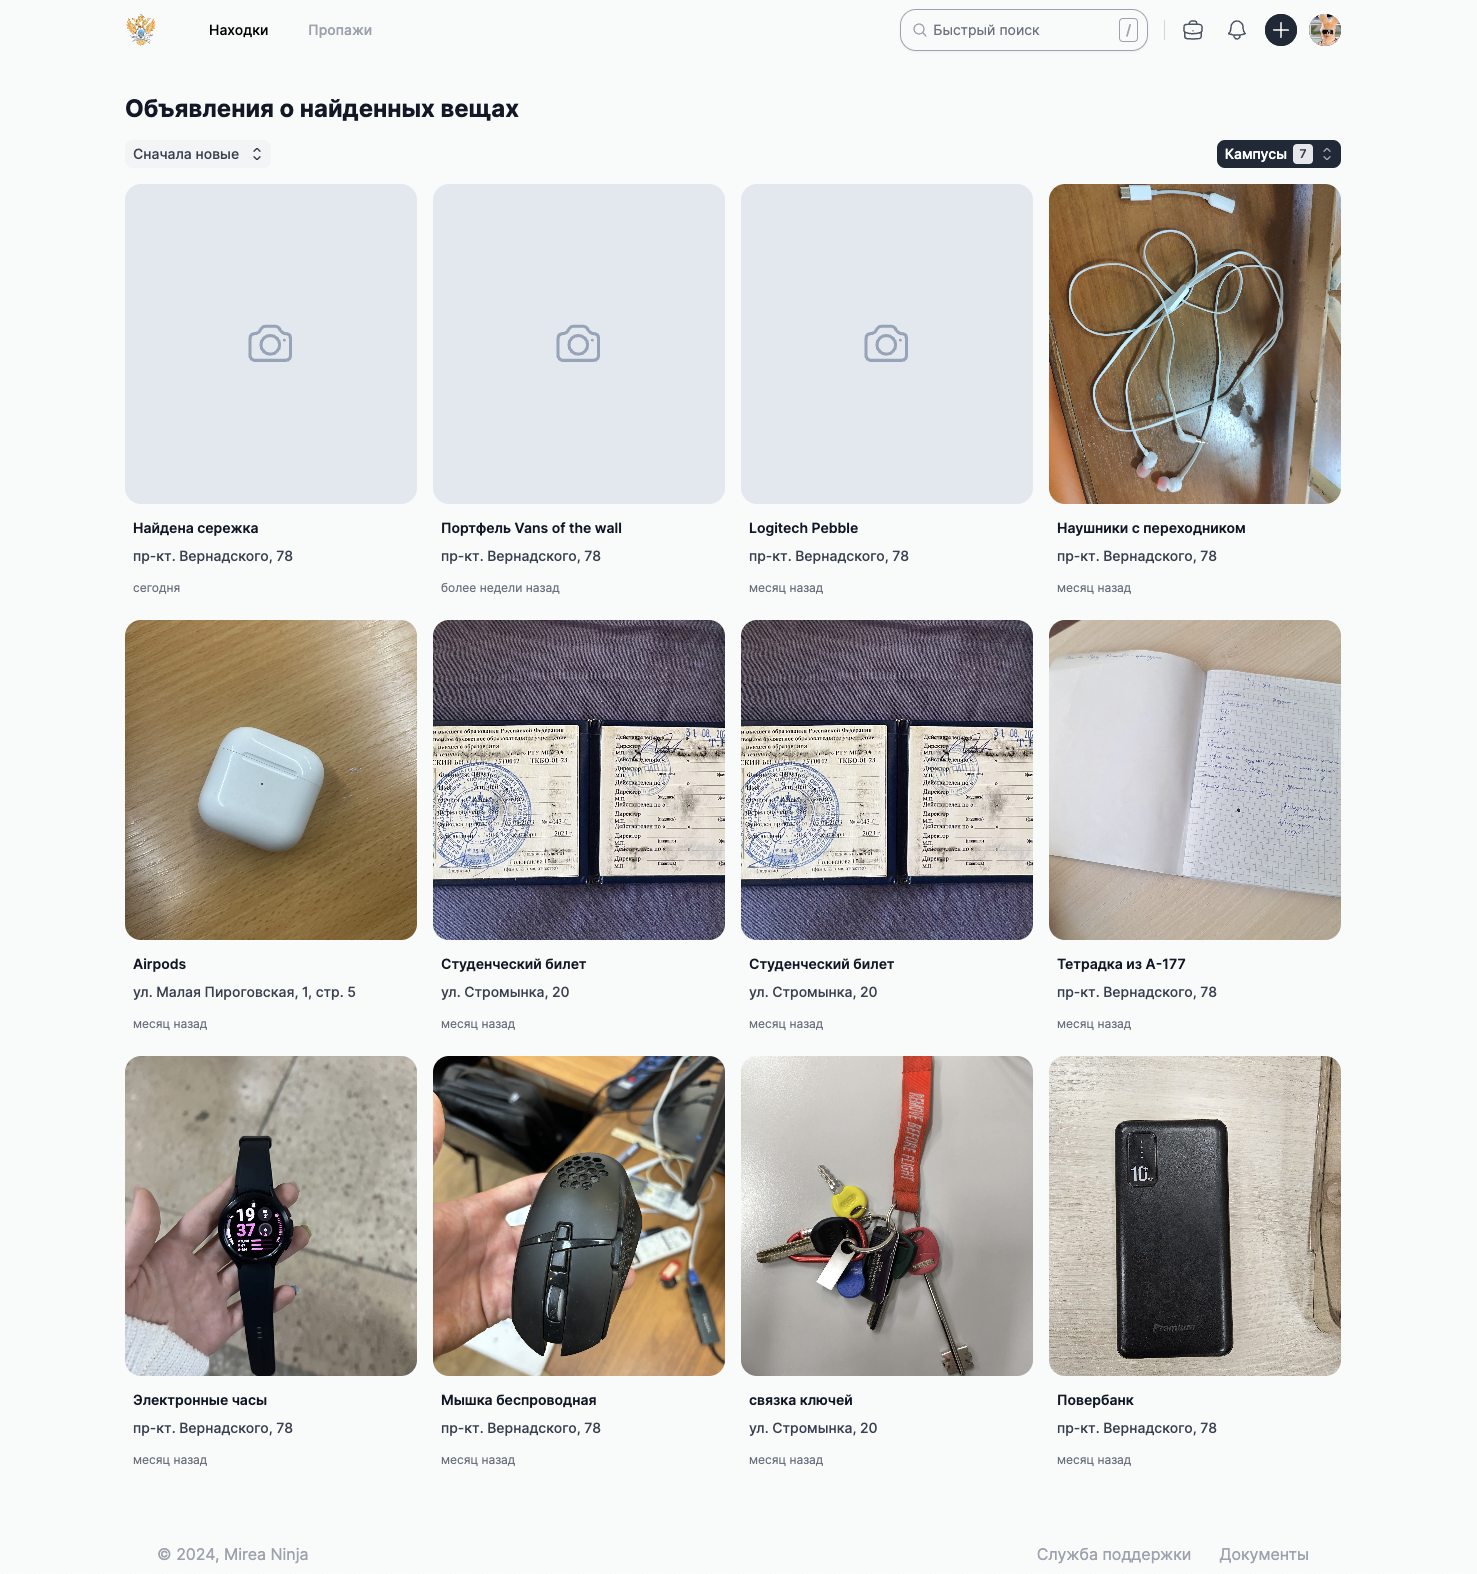
\includegraphics[width=.95\textwidth]{images/infinity-scroll-page.png}
	\parskip=6pt
	\caption{Страница бесконечной ленты объявлений}
	\label{fig:infinity-scroll-page}
\end{figure}

\subsubsection{Модуль добавления и поиска утерянных вещей}

Для добавления утерянных вещей реализована форма с вводом названия, описания, возможностью загружать картинки в объектное хранилище. Форма представлена на рисунке \ref{fig:lost-item-from-page}.

\begin{figure}[htb]
	\centering
	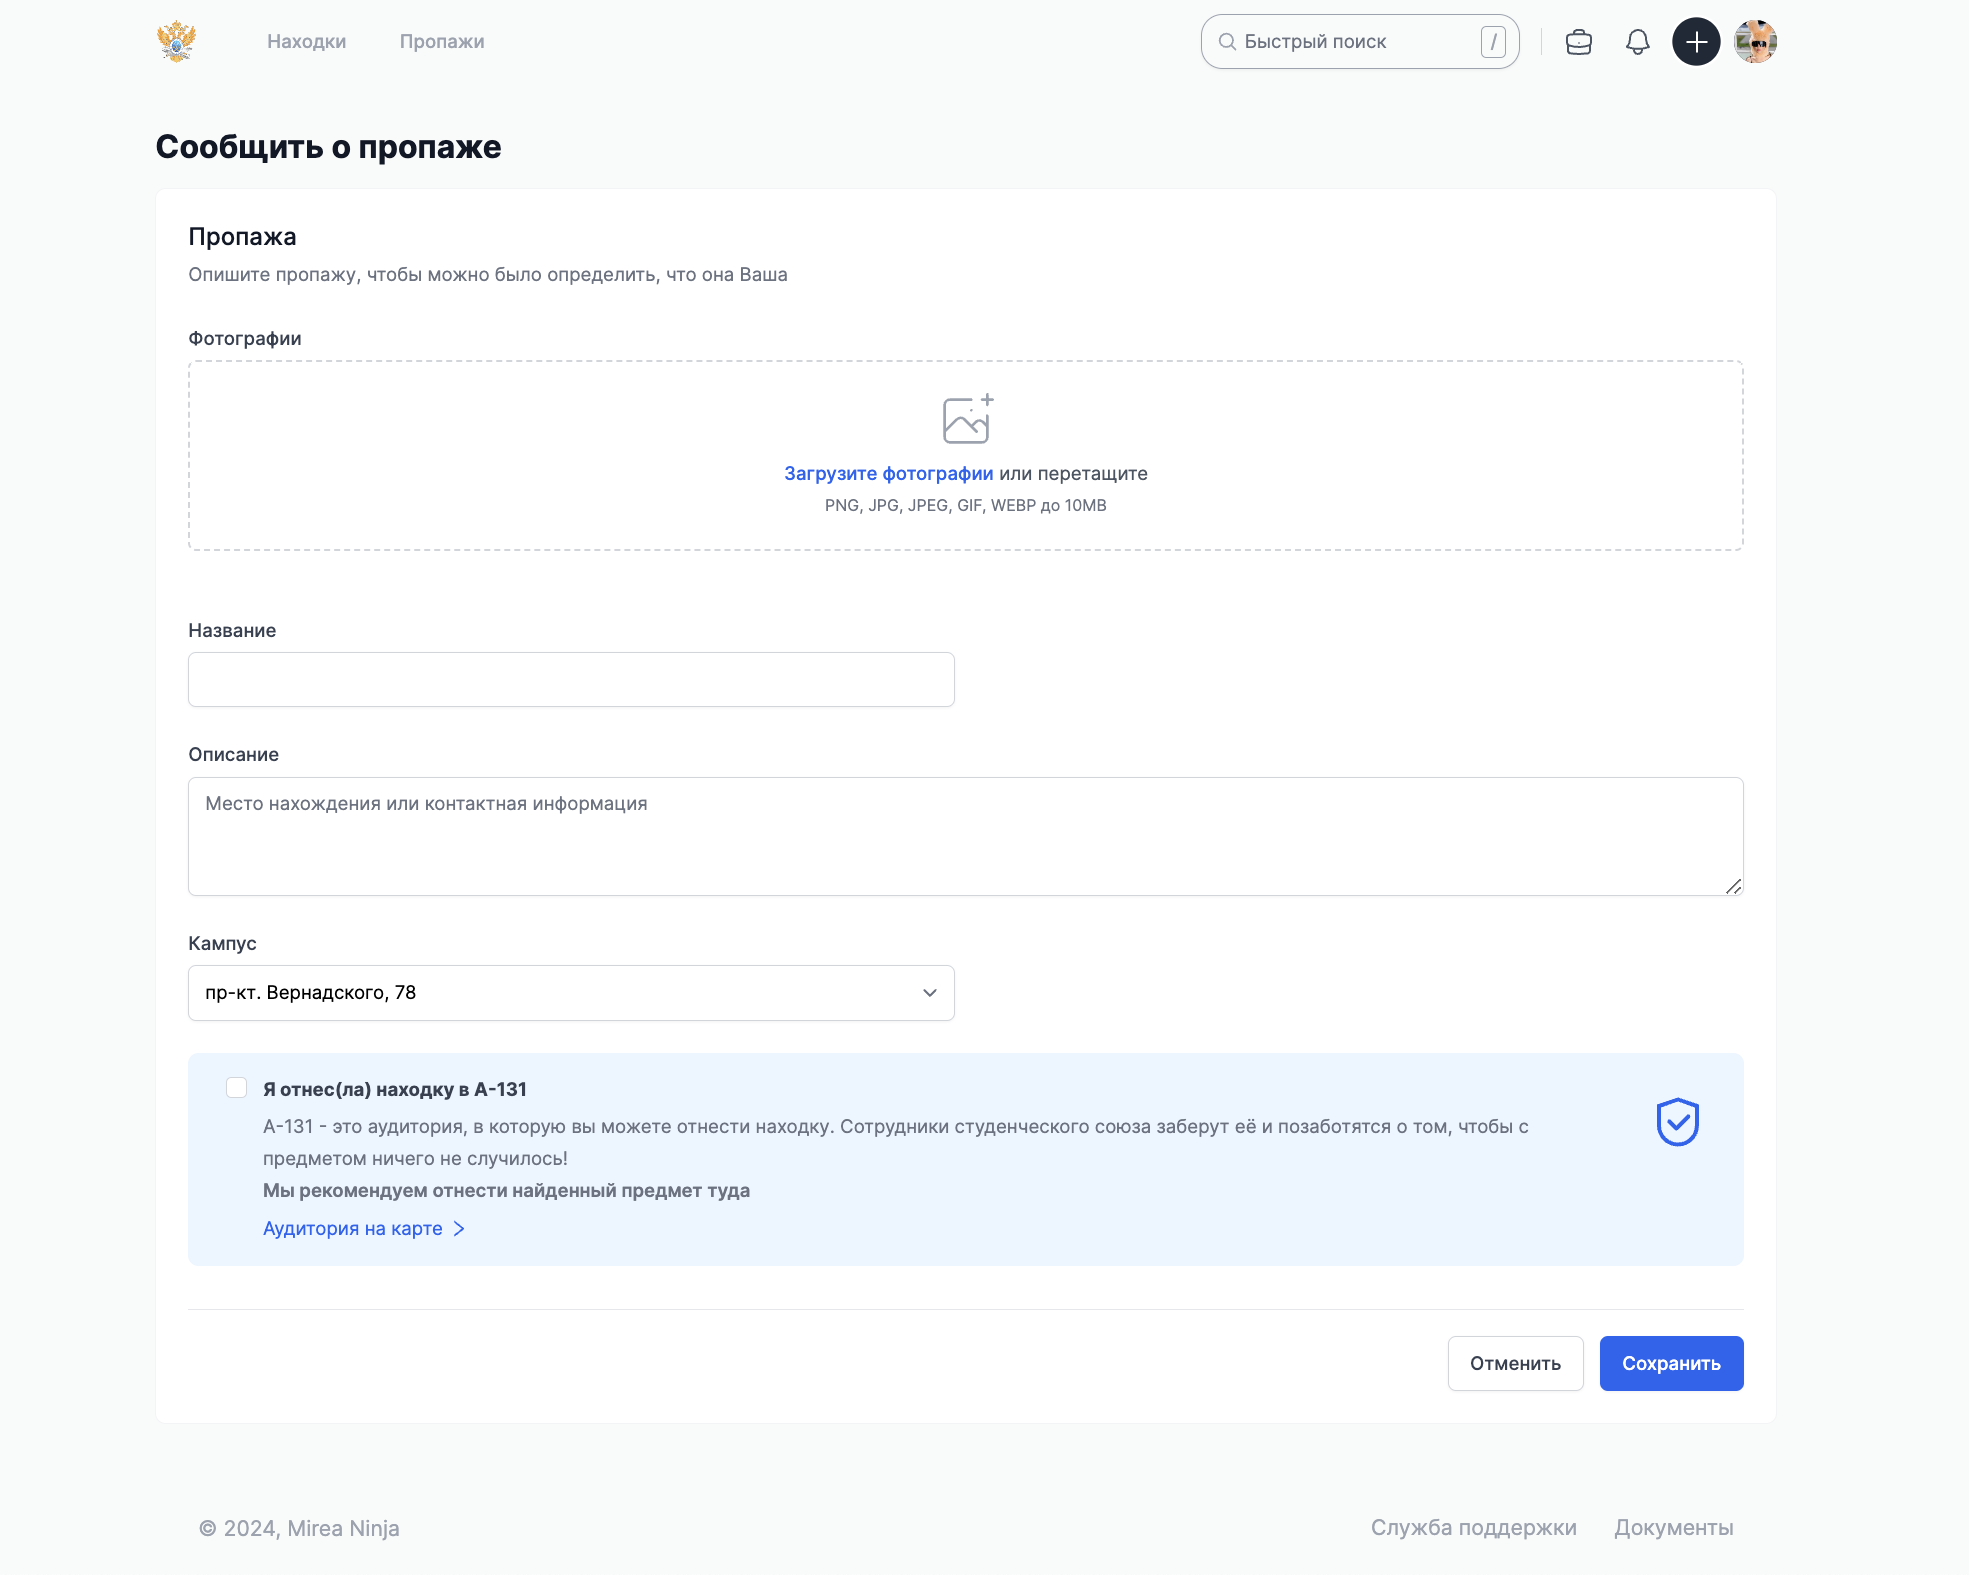
\includegraphics[width=.95\textwidth]{images/lost-item-from-page.png}
	\parskip=6pt
	\caption{Форма ввода утерянных вещей}
	\label{fig:lost-item-from-page}
\end{figure}

Полнотекстовый поиск по названиям и описаниям происходит по названиям и описанию объявлений. Реализация клиентской части поиска представлена на рисунке \ref{fig:search-page}.

\begin{figure}[htb]
	\centering
	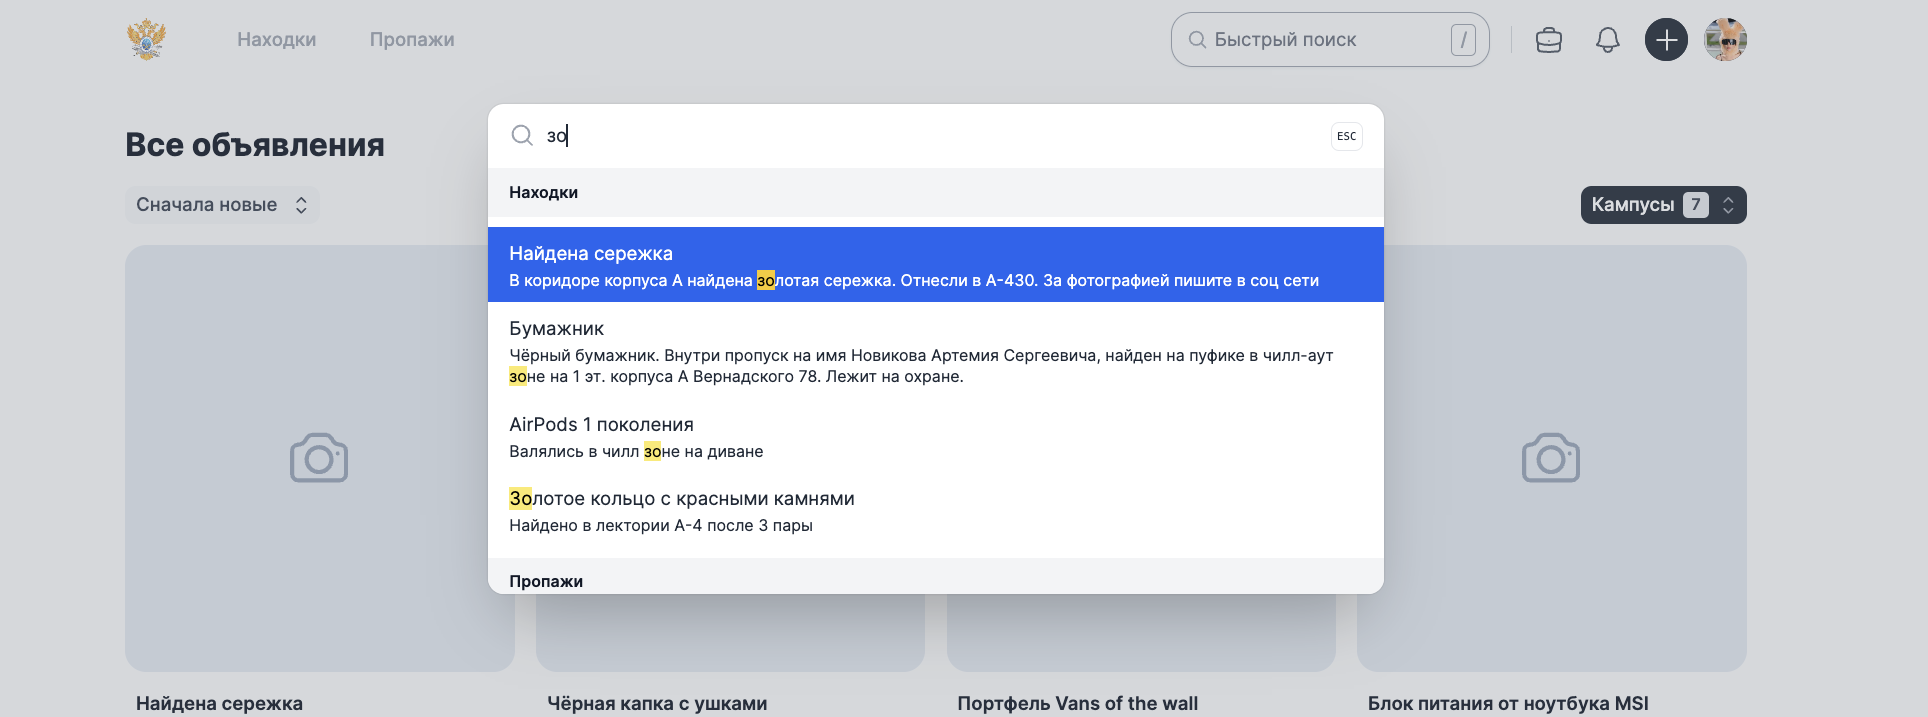
\includegraphics[width=.95\textwidth]{images/search-page.png}
	\parskip=6pt
	\caption{Форма ввода утерянных вещей}
	\label{fig:search-page}
\end{figure}

\subsection*{Вывод по разделу}

Для обеспечения надежности приложения были внедрены механизмы логирования и мониторинга. Это позволяет оперативно выявлять и устранять возможные проблемы, а также анализировать поведение пользователей для дальнейшего улучшения приложения.

В итоге, все эти модули вместе обеспечивают безопасное и удобное функционирование приложения, соответствующее современным стандартам и требованиям.

Поиск утерянных вещей является актуальной проблемой, которая возникает при различных обстоятельствах. Эта проблема может возникнуть в результате потери ключей, документов, мобильных телефонов, кошельков или других ценных или важных вещей. В связи с этим существует необходимость разработки системы, которая поможет людям вернуть утерянные вещи.

Разработка системы для поиска утерянных вещей позволит создать удобный инструмент для поиска потерянных вещей, что приведет к уменьшению количества потерянных вещей и улучшению качества жизни людей. В ходе данной работы были проанализированы существующие системы и технологии, определены требования к разрабатываемой системе и ее функциональности. На основе этого анализа были разработаны и внедрены модули, обеспечивающие высокую безопасность, удобство использования и надежность системы.

Таким образом, итогом работы стало создание комплексного решения, которое решает проблему поиска утерянных вещей, улучшая повседневную жизнь пользователей.